\documentclass[a4paper,12pt]{ctexart}
\usepackage[style=gb7714-2015ay]{biblatex}
\usepackage{graphicx}
\usepackage[scale=0.8]{geometry}
\usepackage{amsmath}
\usepackage{amssymb}
\usepackage{float}
\usepackage[hidelinks]{hyperref}

\providecommand{\keywords}[1]{\\\textbf{\textit{关键词:}} #1}
\addbibresource{reference.bib}
\title{绿色金融推动一带一路发展}
\author{董晨阳}
\date{\today}
\begin{document}
\maketitle
\begin{abstract}
在这里写摘要。
\keywords{一带一路,绿色金融}
\end{abstract}
\clearpage
\section*{引言}

发展中国家往往面临污染权和发展权的权衡取舍\cite{曾文革2012从碳排放权之争看我国在气候变化上的法律应对}。大部分共建“一带一路”国家属于发展中国家,依赖高污染的行业可以使经济短期内粗放式快速发展,但代价却是牺牲环境、牺牲未来长期的发展利益。从自然资源禀赋及产业结构上看,很多“一带一路”国家能源结构相对依赖于传统化石能源,产业相对落后,经济社会发展、实现国家现代化的迫切愿望与追求绿色转型面临两难。如何运用政策和市场工具实现生态保护与经济发展的平衡,实现低排放、高增长的发展路径,对这些国家而言不仅是现实的挑战,也可能带来经济上的负担。
\begin{figure}[H]
    \centering
    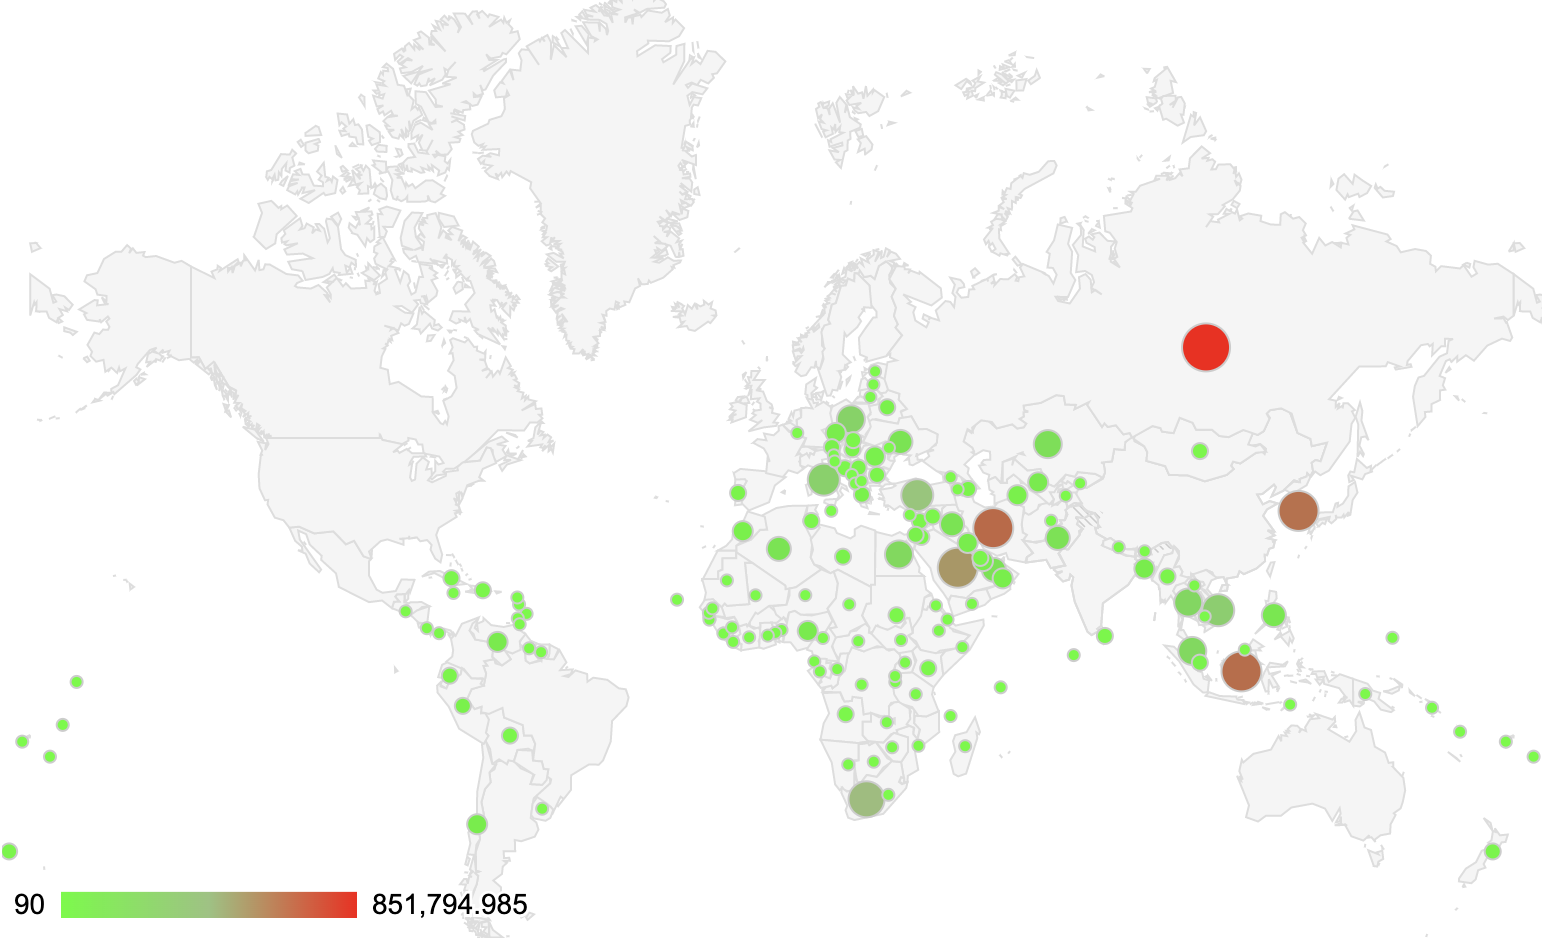
\includegraphics[width=0.8\linewidth]{./img/碳排放.png}
    \label{fig:carbonemit}
    \caption{一带一路国家2019年碳排放。数据来源:世界银行}
\end{figure}

绿色金融是缓解污染权和发展权矛盾的一种手段。绿色金融一种纳入环境因素的金融业务运作、产生环境效益的、服务于可持续发展的金融活动,例如为环境改善、气候变化和资源节约等领域开展投融资、项目运营、风险管理等金融服务,这些领域包括但不限于环保、节能、清洁能源、绿色交通、绿色建筑等领域。
绿色金融一方面意味着金融业要促进环境、经济、社会的可持续发展,能从资金端引导资金流向生态环境保护型产业,能从生产端引导企业生产注重绿色环保,从消费端引导消费者形成绿色消费理念;另一方面也意味着金融业自身的可持续发展,避免注重短期利益的过度投机行为。

通过绿色金融助力“一带一路”国家实现低碳转型具有紧迫性。
2019年,146个共建“一带一路”国家1碳排放总量约占全球30.8\%,显著高于其GDP占全球22.1\%的份额,且近5年增速远高于其它地区。同时,考虑到大部分“一带一路”国家仍处于工业化、城镇化的快速发展阶段,在未来一段时期内,碳排放规模仍将持续上升,可能成为新的“排放大户”。
\begin{figure}[H]
    \centering
    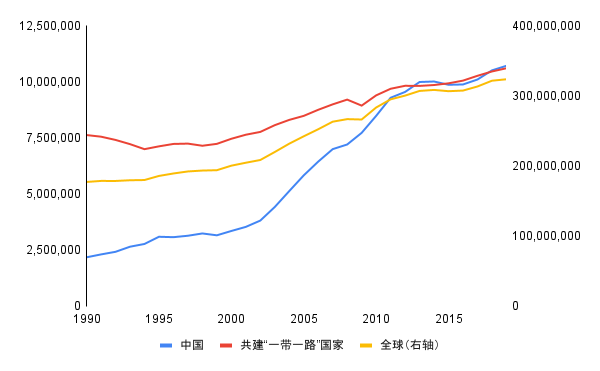
\includegraphics[width=0.8\linewidth]{./img/碳排放-折线图.png}
    \label{fig:carbonemit2}
    \caption{碳排放历史数据。数据来源:世界银行}
\end{figure}

通过绿色金融追求低碳发展也是共建“一带一路”国家的自身诉求。
作为全球应对气候变化的重要参与者,大部分“一带一路”国家积极支持和推动应对气候变化国际合作进程,参与多边框架谈判和国际规则制定,并在联合国气候变化框架公约下提交国家自主贡献承诺,在绿色能源、绿色建筑、绿色农业等领域提出相应的行动举措。
“一带一路”国家的生态环境相对脆弱、环境承载力不高,受全球气候变化影响和冲击可能更大,其率先实现绿色发展也更具紧迫性。

因此,通过绿色金融助力“一带一路”国家实现绿色转型具有充分的必要性和重要性。

\section*{文献综述}
关于绿色金融的定义,学界虽然没有统一的定义,但有一致的内涵,即联系起经济发展与环境保护,保持经济的可持续发展\cite{雷立钧2009绿色金融文献综述}。\citet{cowan1998topical}认为绿色金融是一种环境学和金融学的交叉学科,\citet{gray2002messiness}则认为是将社会与环境因素加入到金融学中,\citet{hohne2012mapping}认为绿色金融的内涵是随时间变化发展的,其定义取决于可持续性项目、环境政策等的定义。\citet*{张承惠2016发展中国绿色金融的逻辑与框架}则认为发达国家的定义偏重气候,由于他们已经完成了工业化,因而其认为即便是化石能源的更高效利用也不属于绿色金融;发展中国家则强调了发展属性,只要能够节约化石能源的使用量、降低单位能耗,相关投资都属于“绿色”
\begin{figure}[H]
    \centering
    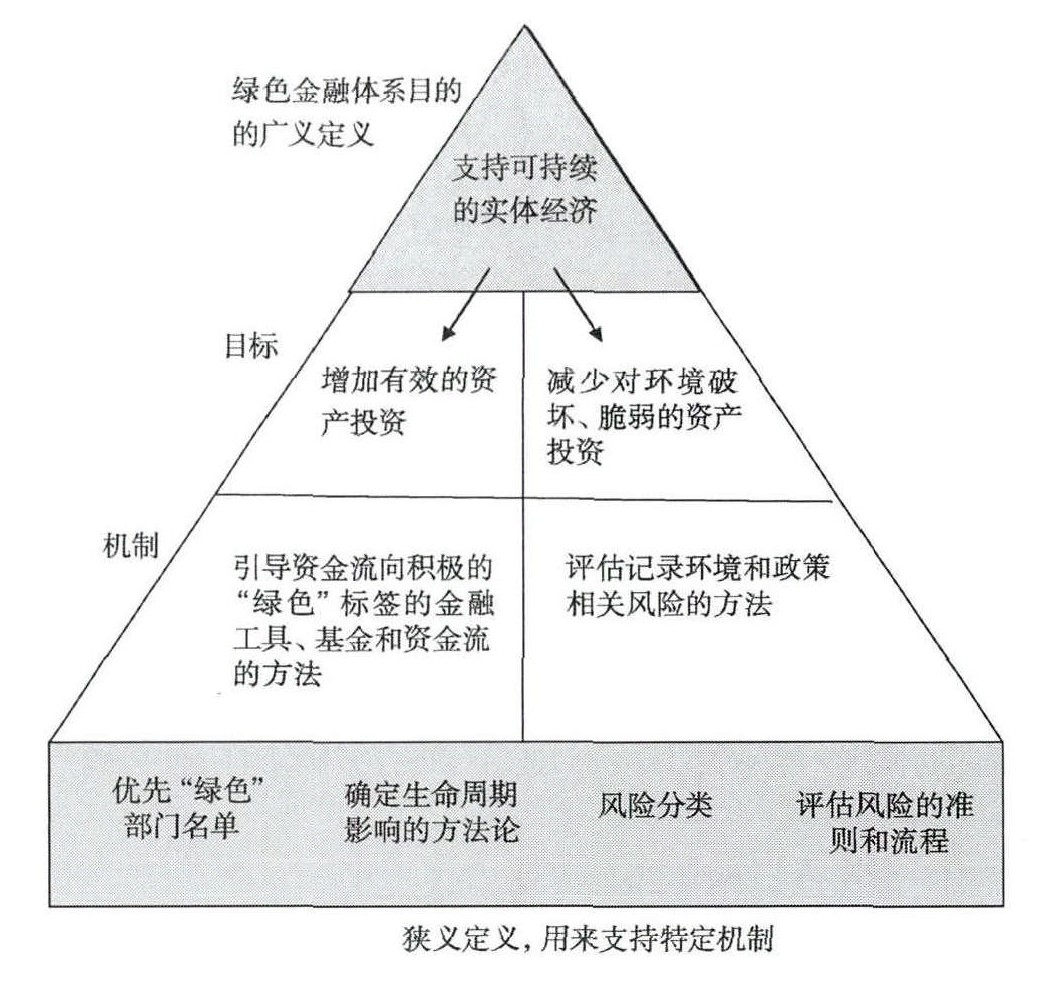
\includegraphics[width=0.5\linewidth]{./img/绿色金融定义.jpeg}
    \caption{绿色金融的定义。资料来源:联合国环境规划署}
\end{figure}

绿色金融的意义

绿色金融工具主要在绿色金融市场中体现,绿色金融市场主要有绿色风投、绿色债券市场、绿色债券市场、碳金融市场与绿色保险市场\cite{姚秋池2017国内外绿色金融研究综述}。

\section*{国内外关于绿色可持续发展的相关政策}

\section*{绿色金融潜在市场规模估测}

\section*{结论与建议}

\nocite{*}
\printbibliography
\end{document}
